\subsection{Impacts of the applied force}
In setup 3 and setup 4 each protein was stabilized with an external force acting on the FERM domain (see \autoref{motivation}). These forces have of course impacts on the FAK molecules, which are analysed below.\\
The force itself has a mean value of $1.47\,\forceunit$ and a standard deviation of $13.13\,\forceunit$. It is skewed to positive values, which was expected as deviations with a negative sign are restricted due to $z_0 + \Delta z \le d_F$ (see below). Neither additional maxima nor minima are observable in its distribution.
\subsubsection{Distance between F1 and F2}
First the COM distance of F1 and F2, namely $d_F$, is considered. In \autoref{force:distcorr} a hexbinning plot of $d_F$ against the force can be found. The plot shows, that some combinations (below the orange line) are never visited. For a given force, $d_F$ seems to have a lower boundary. This boundary is defined by $d_{F, \text{min}} = z_0 - \Delta z$, where $z_0$ is the reference distance of the force and $\Delta z$ the elongation (proportional to the force), and is reached, if the vector between F1 and F2, $\vec{d}_F$, is parallel to the z-axis.\\
The plot indicates, that $d_F$ and the force are hardly correlated, which is tested with a linear regression. In order to not bias the regression by $d_{F, \text{min}}$ only points with a force lower than $0\,\forceunit$ are taken into account. With a p-Value of $23\%$ for the H0 hypothesis slope $m = 0$, the distance $d_F$ and the applied force can indeed be seen as uncorrelated.
%
%
%
\begin{figure}
	\centering
	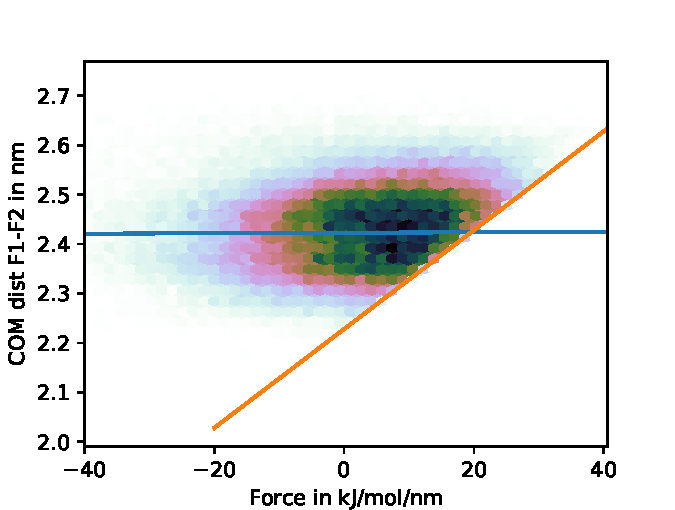
\includegraphics[width=.5\textwidth]{figures/results/force_forcef1f2}
	\captionof{figure}{$d_F$ against the force. The orange line defines the minimum value of $d_F$. The blue line shows the result of the linear regression.}
	\label{force:distcorr}
\end{figure}
%
%
%
%
%\subsubsection{Inclination angle of FAK}
% TODO: important?
%The applied force is directly linked to the angle between the distance vector of F1 and F2 and the z-axis, namely $\beta$. In order to examine how much the forces bias $\beta$, the distribution of $\beta$ for setup 3 (with external force) are compared to equivalent simulations except the stabilizing force (simulations mentioned in \autoref{motivation}).\\
%The distribution of is very similar to those obtained for the unbiased systems, albeit the mean value is determined by the choice of $z_0$. The variance for the biased system is about $18\,\si{\deg}$ and similar to those of the unbiased systems. This indicates, that the fluctuations around the mean value are not restricted crucially by the applied force.\\
%\\
% TODO: important?
%Since protein dimers are investigated in the following sections, also the distribution of the forces for the different dimer types should be considered. In \autoref{tobeadded} the forces, which occurred on the different dimers, are presented as boxplots. % number of datapoints in description?
%The forces acting on a type 1 protein pairs (FERM-FERM) as well as these acting on a type 3 protein pairs (FERM-kinase) are symmetrically distributed around the overall mean. In contrast the forces acting on e.g. type 9 protein pairs are systematically lower than those acting on other types, which has to be taken into account when analysing those dimers.\\
%One important reason for this can be the sampling. While there are 1 162 144 datapoints for type 1 pairs coming from several different proteins, only 464 datapoints exist for type 9 pairs, mainly observed in one pair only.\\
%\\
\subsubsection{Intramolecular distances}
%TODO: check also CA
\label{forceana:intramolec}
First all distances between interacting residues are tested on correlation with the applied force. For this 10 different proteins without neighbours were picked out of the trajectories from setup 4, each for $1\,\si{\micro\second}$. In \autoref{force:contactmap} the calculated Pearson correlation coefficients for significant correlations are shown. There are 270 residue pairs contributing to the interface, which show a large correlation (Pearson $\left|r\right| > 0.3$). The calculated slope of these pairs is $\approx \pm  20 \text{force unit}/\si{\nano\metre}$. A change of the force of one standard deviation would therefore lead to a change of roughly $0.6\,\si{\nano\metre}$. Furthermore spots exists, which show the same sign in the correlation. Thus the force can have large influences on the interface.\\
Also the COM distances between F1 and the N-lobe as well as F2 and the C-lobe were tested upon correlation with the external force using a linear regression. Both reveal a significant correlation, but the maximum obtained slope is $0.0008\, \si{\nano\metre}/\text{force unit}$. Changes in the distance upon the external force can therefore be neglected.
%
%
%
\begin{figure}
	\centering
	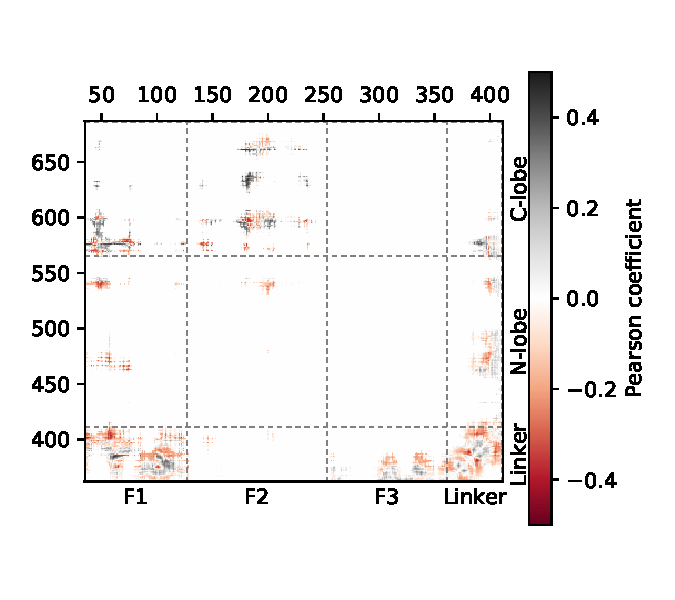
\includegraphics[width=.7\textwidth]{figures/results/interface_corr}
	\captionof{figure}{Correlation of residue-residue distances upon external force}
	\label{force:contactmap}
\end{figure}
%
%
%
\\
It is important to see, that in this section only the observed quantities were tested for correlation with the force. It is however possible and probable, that due to the restriction, configurations or states are completely missing while others become over expressed. This effect can not be estimated, but should be kept in mind.